
% {{{ preamble

\documentclass{article}

\usepackage{url}
\usepackage{hyperref}
\usepackage{graphicx}
\usepackage{nonfloat}
\usepackage{amsmath}
\usepackage{fancyvrb}
\usepackage{parskip}
\usepackage{color}

\usepackage{courier}
\usepackage{listings}
\lstset{numbers=left,
		language=C,
		tabsize=4,
		basicstyle=\ttfamily,
		columns=fixed,
		%basicstyle=\footnotesize,
		showstringspaces=false,  % don't show the space character
		%commentstyle=\textit,
		showtabs=false,
		extendedchars=true,
		basicstyle=\normalsize,
		captionpos=b,
		frame=tb,
		xleftmargin=0.3in}

\usepackage{vmargin}  % make the margins a bit smaller
%\setmarginsrb{1.0in}{1.0in}{1.0in}{1.0in}{0in}{0.4in}{0.0in}{0.40in}
\setmarginsrb{1.0in}{1.0in}{1.0in}{1.0in}{0in}{0.25in}{0in}{0.20in}

\raggedright

\usepackage[backend=biber,autocite=footnote,
			bibstyle=authortitle,citestyle=verbose-inote]{biblatex}
\setlength{\bibitemsep}{\baselineskip}

\addbibresource{main.bib}

\providecommand{\e}[1]{\ensuremath{\times 10^{#1}}}

% }}}

\begin{document}

\VerbatimFootnotes

% {{{ title page

\thispagestyle{empty}

\centerline{\Large \textbf{SprinklerPI}}
\vspace{0.1in}
\centerline{\normalsize {Jeremiah Mahler} ({\href{mailto:jmmahler@gmail.com}{jmmahler@gmail.com}})}
\centerline{\small \today}
\vspace{0.2in}

% }}}

%\tableofcontents
%\pagebreak

% {{{ Introduction
\section{Introduction}

The task of watering your lawn is conceptually simple.
Turn on certain sprinklers at certain times and run them for
a certain duration.

The well known UNIX/Linux program \verb+cron+ can run any program
on any schedule: every day, every other day, every third Friday,
every day during the month of august.  The possible combinations
are endless.

Using the power of \verb+cron+ on a RasberryPI\autocite{rasberrypi}
running Linux with a small amount interface hardware to control the
sprinkler valves and the result is a very powerful sprinkler control system.

% }}}

% {{{ Control
\clearpage
\section{Control}
\label{sec:control}

Before the sprinkler valve can be driven, some control logic is necessary
between the RasberryPI and the driver (Section \ref{sec:driver}).
Most residential sprinkler systems are capable of driving eight circuits.
And only one of these circuits can be active at any one time
\footnote{If multiple circuits were active this could lower the
water pressure resulting in inconsistent watering amounts.}.
This controller uses the same design
\footnote{With some minor redesign this controller could be
expanded to control a large number of circuits possibly
with multiple active circuits at a time.}.

The RasberryPI has enough GPIO pins to control each valve independently.
But doing this would be a waste.
Future expansion to a large number of circuits would be severely limited.
And the time requirements are very generous.
Being able to switch a valve every second is more than adequate.

Instead of using individual GPIO pins, the four SPI pins provided by
the SPI are used.
This design sends 8-bits for each message (Figure \ref{fig:spi}).
But only three bits are used to address each valve ($2^3 = 8$).
If the design was expanded to use the available bits
it could address 128 valves ($2^7 = 128$).
The single enable bit was chosen to simplify the circuitry.
However it does reduce the maximum number of addresses by one bit.

{
\renewcommand*\arraystretch{1.5}
\begin{figure}[hbp]

\centering
\begin{tabular}{l r l r l r }
7 & 4 & 3 & 1 & \multicolumn{2}{c}{0} \\
\hline
\multicolumn{2}{|c|}{\hspace*{6mm} unused \hspace*{6mm}} &
\multicolumn{2}{|c|}{\hspace*{4mm} valve \hspace*{4mm}} &
\multicolumn{2}{|c|}{\hspace*{1mm} en\_n \hspace*{1mm}} \\
\hline
\end{tabular}

\caption{SPI message format.}
\label{fig:spi}
\end{figure}
}

Going from SPI to signals which can turn on/off a valve requires
more logic than has been discussed so far.
A shift register is needed to take the bits as inputs.
A decoder is needed to convert shifted in number to a single
bit output.
In this case a 74HC238 3-8 decoder is used since it provides non-inverting
inputs suitable from the drivers (Section \ref{sec:driver}).
An output high will turn on a valve.
Figure \ref{fig:control} shows the control schematic.

\begin{figure}[hbp]
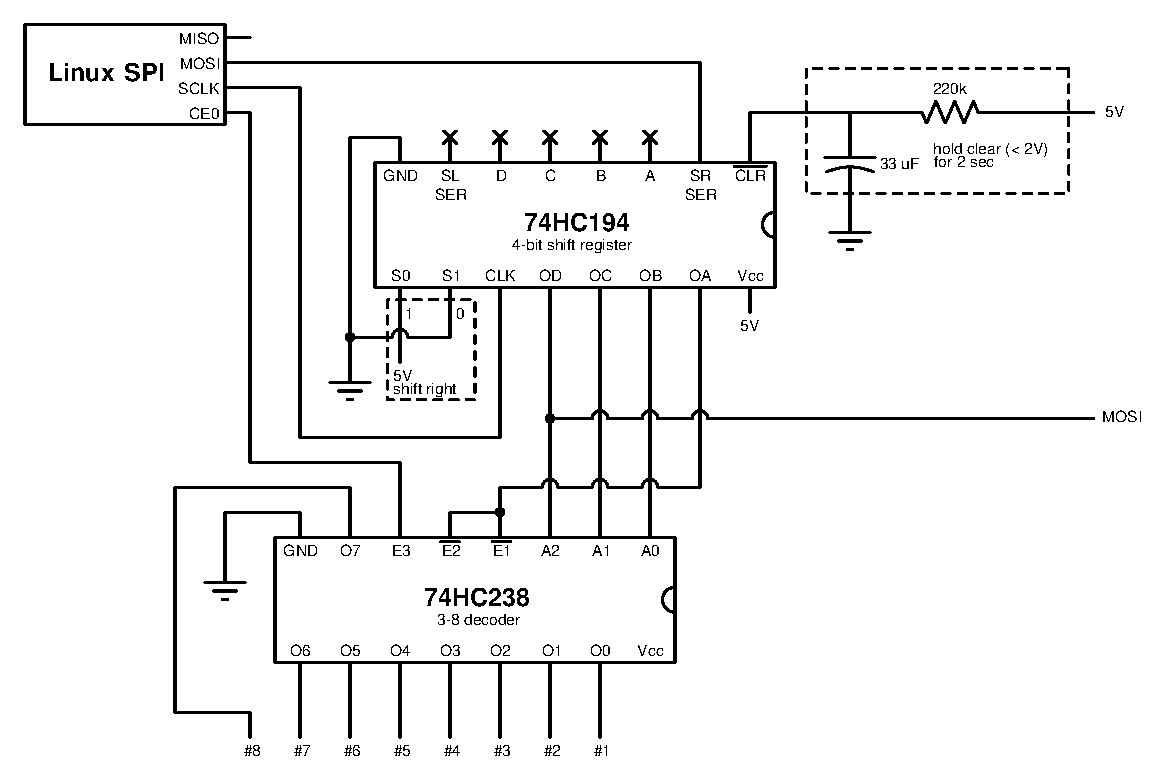
\includegraphics[scale=0.90]{xcircuit/control}
\caption{Sprinkler valve control logic.
Sprinkler valve number is input using SPI from the RasberryPI in
to the shift register.  The number is decoded and inverted to produce
a single high signal for one valve.
All outputs are disabled when OA is clear.}\label{fig:control}
\end{figure}

On power up it is important that the valves remain off.
However the shift register chip (74HC194) does not guarantee
the output state during power up.
To resolve this issue a simple RC circuit is used to to hold the
chip in the clear state for several seconds after power
on (Figure \ref{fig:control}).

% }}}

% {{{ Driver
\clearpage
\section{Driver}
\label{sec:driver}

\begin{figure}[hbp]
\centering
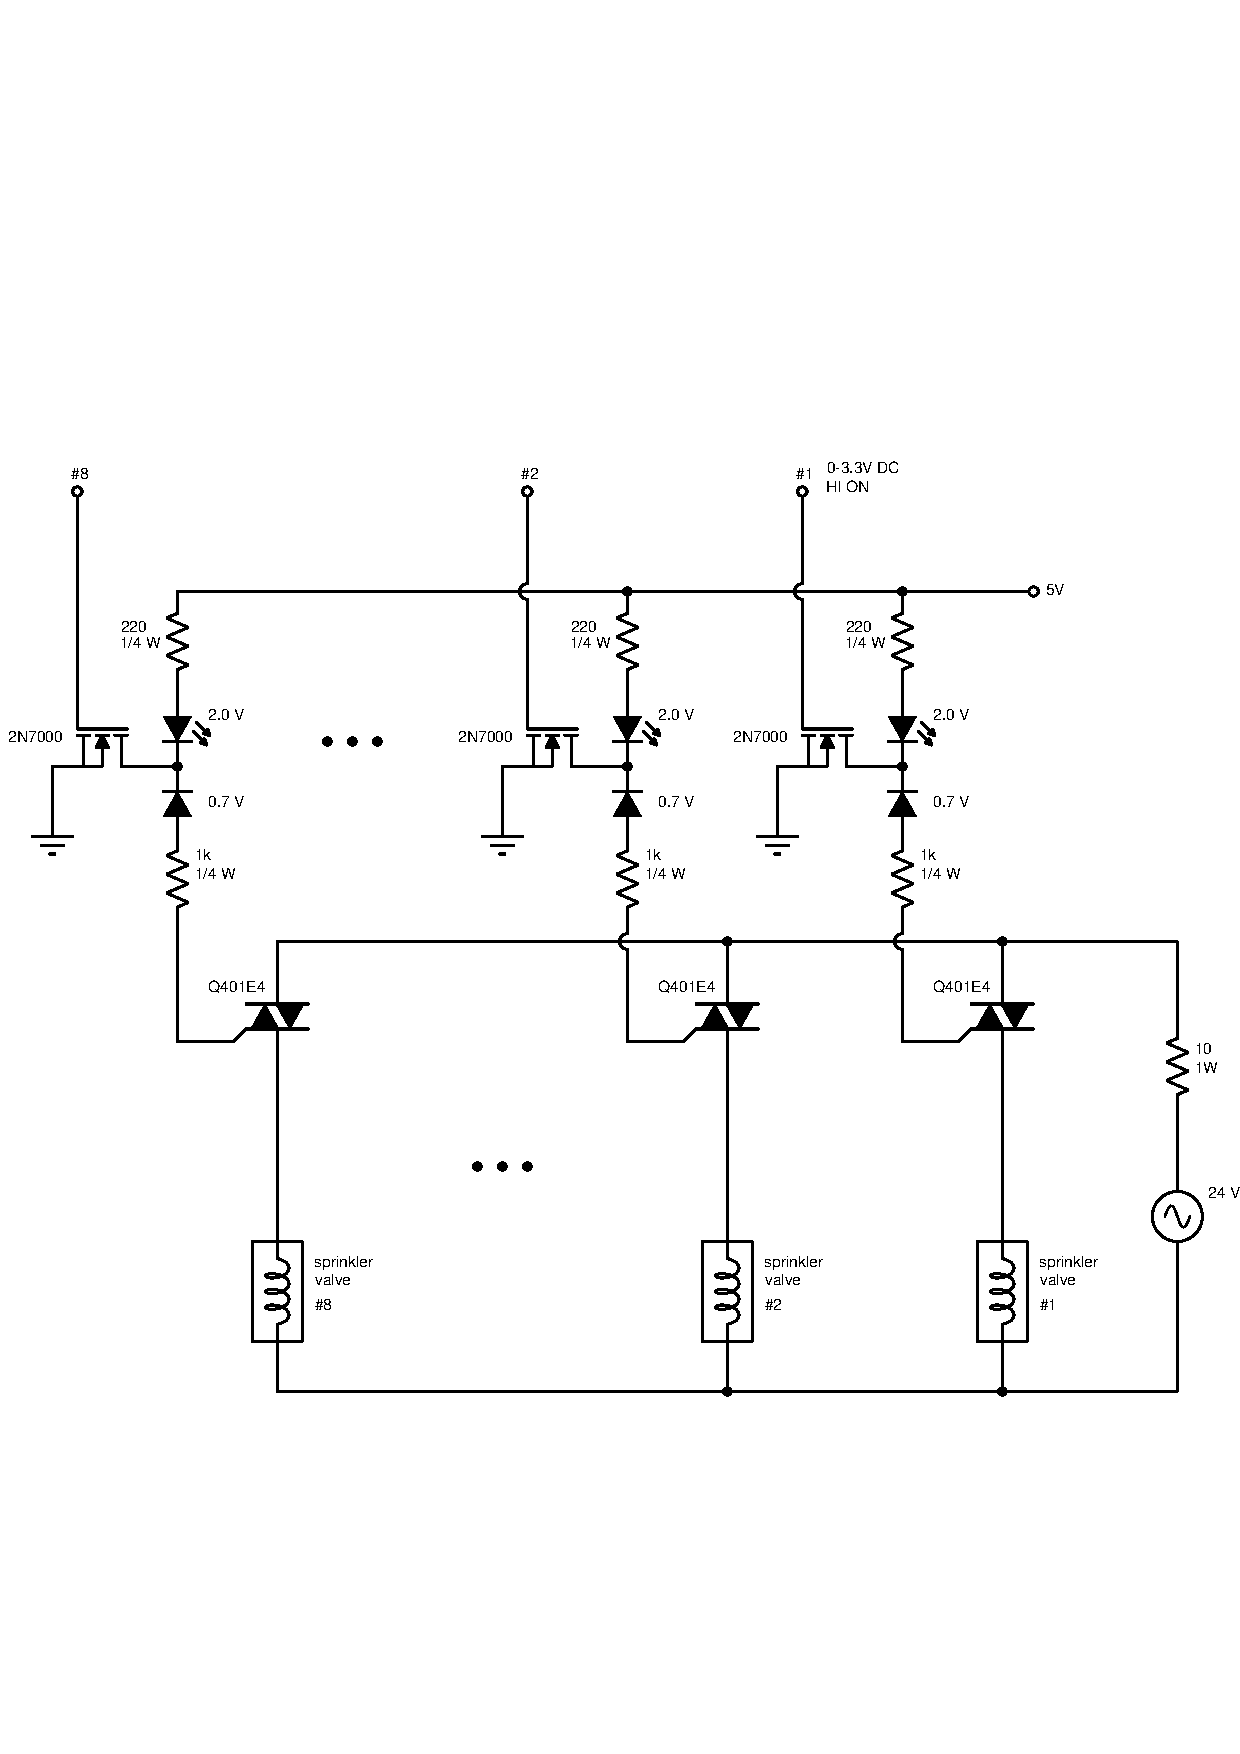
\includegraphics[scale=0.7]{xcircuit/driver_mult}
\caption{Sprinkler valve driver circuits.  For brevity not
all drivers are shown since they all have identical designs.
LEDs are used to indicate when the valve is on/off.
This design assumes that only one valve will be one at a time.
}\label{fig:driver}
\end{figure}

To turn the sprinkler valves on requires 24 VAC at approximately 270 mA.
If it is assumed that during steady state both the solenoid
and the triac have negligible resistance (Figure \ref{fig:driver}),
a 10 $\Omega$ resistor can be used to limit the current to 240 mA.
At 1 watt the resistor supports the worst case amperage with a margin
over 10\%.

\begin{align*}
	P &= I^2 R \\
	  &= (270\e{-3})^2 \cdot 10 \\
	  &= 0.729 \quad \text{[W]}
\end{align*}

The control signal to the triac (Q401E4) is very sensitive.
The tinyest current will cause it to conduct.
If it is driven by a 0-5V signal it will conduct not only
with a 5V signal but also with 0V signal.
To overcome this issue a diode was used to ensure no current
flows when it is reverse biased.
The FET (2N7000) is used to switch the triac while it also
serves to limit the control current of a 0-5 volt signal
to less than 0.5 mA.
This places the control current well within the limits
of CMOS logic as required by the control chips (Section \ref{sec:control}).

% }}}

% {{{ Power Supply
\clearpage
\section{Power Supply}
\label{sec:power}

The power supply must provide two different voltages: 24 volts AC and
5 volts DC.
The sprinkler valves require 24 volts AC at 270 mA.
The RasberryPI and other digital logic require 5 volts DC with a
maximum draw of 600 mA
\footnote{The current draw of the RasberryPI was determined
experimentally to be approximately 500 mA.}.
These voltages must be created from a 110 volt AC input.

The 24 volts AC can be achieved using a split pole transformer
with two 12 volt AC outputs.
By bridging the center of these two 12 volt AC outputs
a combined 24 volt AC output is available.

A switching voltage regulator, the MC34063A, was chosen for
the 5 volt supply.
It has a greater efficiency than a linear regulator such as
the LM7805.

The circuit which achieves all of these design requirements is
shown in Figure \ref{fig:power}.

\begin{figure}[hbp]
\centering
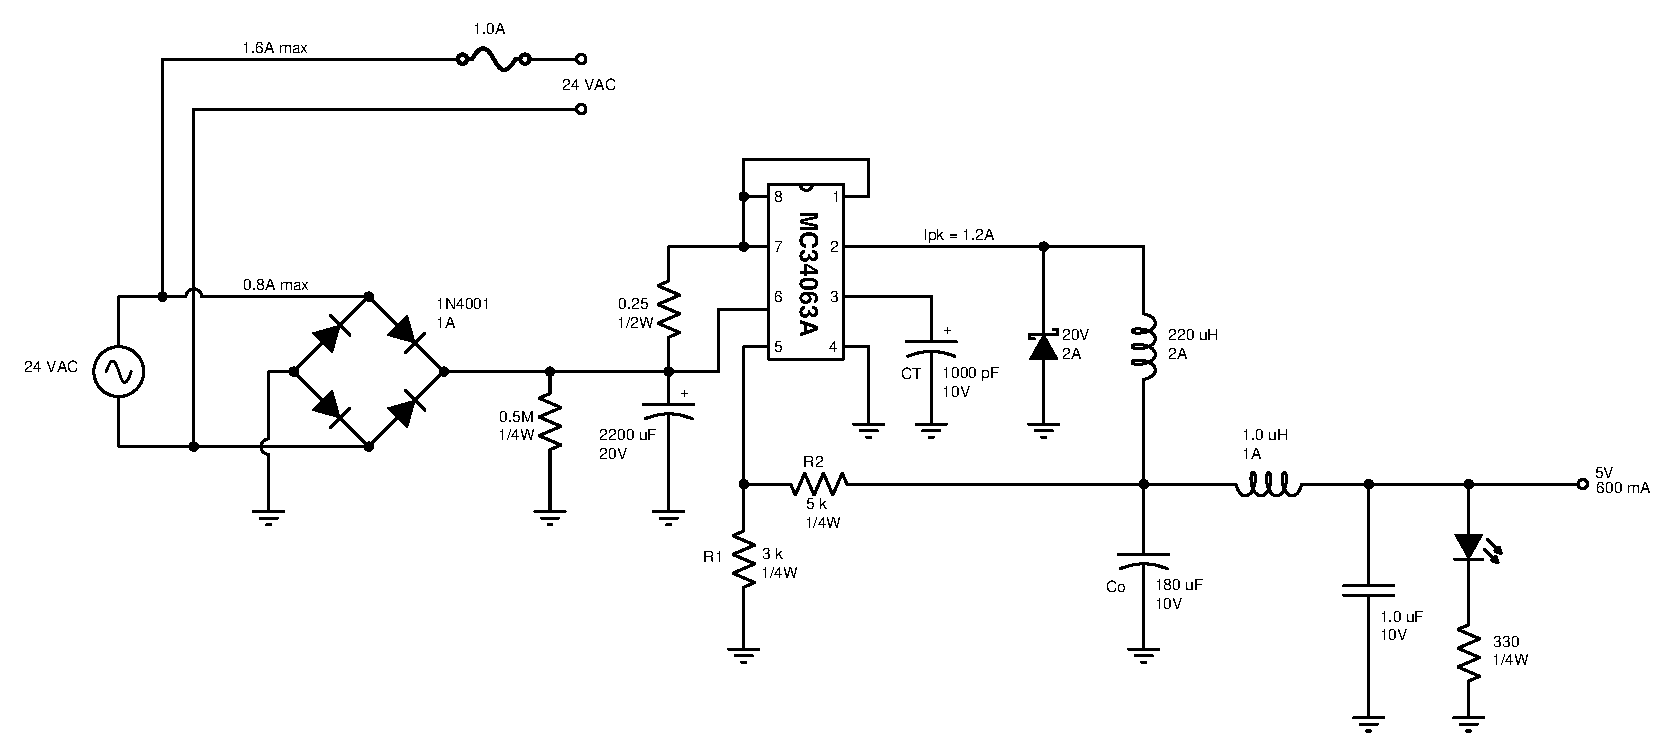
\includegraphics[angle=90,scale=0.80]{xcircuit/power_supply}
\caption{Power supply circuit. A 24 volt AC and 5 volt DC output are
provided.  The 5 volt DC is provided by the MC340363A switching
regulator.}\label{fig:power}
\end{figure}

% }}}

% {{{ Expansion
\clearpage
\section{Expansion}
\label{sec:expansion}

The RasberryPI uses SPI to communicate with the
control logic which which drives the sprinkler valve.
Each group can control up to eight valves with one valve
being on at a time.
A daisy chain arrangement can be constructed to allow SPI
to communicate with more than one group as shown in
Figure \ref{fig:expansion_spi}.

\begin{figure}[hbp]
\centering
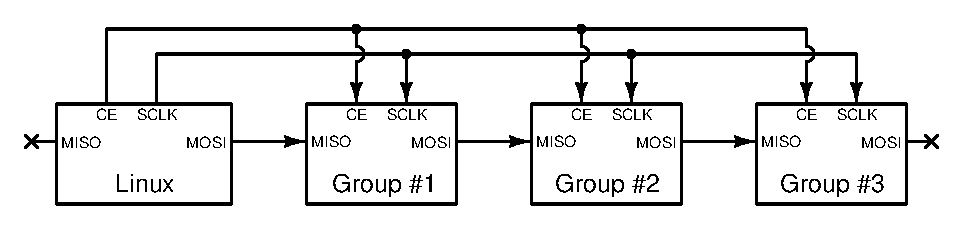
\includegraphics[angle=0,scale=0.80]{xcircuit/expansion_spi}
\caption{Daisy chain SPI configuration to for multiple control groups.
}\label{fig:expansion_spi}
\end{figure}

With the current power supply design it is limited to three
control groups as shown in Figure \ref{fig:expansion_current}.
Each group can control eight valves with one being on at a time.
This makes a total of 24 valves where three can be on at once.

\begin{figure}[hbp]
\centering
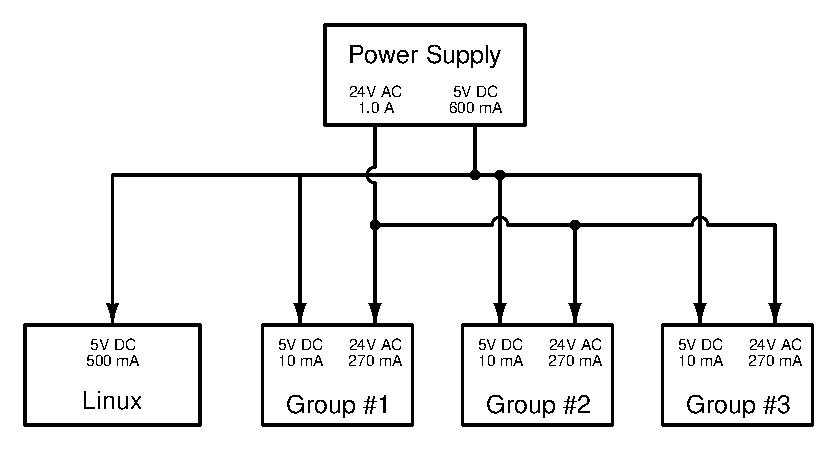
\includegraphics[angle=0,scale=0.80]{xcircuit/expansion_current}
\caption{With a power supply capable of 1 amp at 24 volts AC and
600 mA at 5 volts DC a maximum of three control groups and one
Rasberry PI can be driven.}\label{fig:expansion_current}
\end{figure}

% }}}

\pagebreak
\printbibliography

\end{document}
